\section{Introduction}

A \emph{pangenome} models the full set of genomic elements in a given species or clade \cite{sigaux2000cancer}.
Pangenomics thus stands in contrast to standard genomics by emphasizing the sum total of available genomic information over a particular consensus model of the genome.
By considering the pangenome during bioinformatic analyses, researchers can hope to remove bias towards any specific genome or haploid genome model and incorporate information about genomic variation directly into their study.
%Pangenomic reference systems thus e single canonical version of the genome of a given species, but a widely-represenative collection of sequences.

This concept has been essential to microbiology, where genomic plasticity and diversity have made a pangenomic perspective indispensable \cite{tettelin2005genome,medini2005microbial}.
Usually, these analyses focus on the presence or absence of genes from given strains and the determination of a core (commonly present) and accessory (frequently absent) pangenome \cite{page2015roary}.
Pangenomic techniques have also been applied outside of microbiology, such as in species contexts where genomes are small and often homozygous \cite{cao2011whole}, or in the publication or analysis of collections of novel sequences from a single species \cite{gao2019tomato,brohammer2018maize}.
In recent years, reduced sequencing and \emph{de novo} assembly costs have supported the discovery of significant levels of large-scale genomic variation in many eukaryotic species, including humans \cite{li2010building,sudmant2010,sudmant2015integrated,chaisson2018multi,Yang_2019}, arabidopsis \cite{alonso2016arabidopsis}, brewer's yeast \cite{yue2017contrasting}, and the fruit fly \cite{chakraborty2018hidden}.

These trends encourage the application of pangenomic methods to settings where more than one individual is being analyzed \cite{computational2016computational}.
\todo{JME: I don't understand the logical transition to talking about multiple individuals here. How does this follow from cataloging variation in eukaryotes?}
However, most ``high-throughput'' analyses of large genomes still depend on comparison of individuals to a common reference genome.
This expendient and conservative approach has its merits, but will become untenable with the development of true pangenomic references for humans and other model organisms.
But, to be a true replacement for resequencing, methods based on reference pangenomes must provide precise resolution of variants of all scales, and they must support efficient pangenomic generalizations of many standard bioinformatic approaches.

Here, we consider a new class of methods that approach the pangenome with precision, often at the resolution of single base pairs.
Unlike widely-applied pangenomic methods which consider genes as their fundamental unit, these precise pangenomic methods support the interrogation of collections of genomes and their relationships at any level of resolution.
They envision pangenomic analyses based on the full complement of DNA in the individuals under analysis, and aim to support downstream inference over variants of all types and scales, including small variation such as SNPs and indels in the same context as large structural variants gene gain or loss.

Scaling such techniques to operate on eukaryotic pangenomes has required significant effort in the development of new data models and algorithms.
Solutions to this problem are varied, but they often rely on graph data structures that represent compressed versions of genomes and embed the many-to-many relationships inherent in the pangenome.

Not all methods expose this data structure as a coherent reference system.
They may instead use it internally to improve performance of a standard bioinformatic operation.
Even pangenomic models based on graphs are not necessarily equivalent, and many feature limitations prevent them from representing certain kinds of genomic variation.

Although, these limitations have appeared expedient or even necessary to scale precision pangenomics to eukaryotic genomes, new algorithms and approaches for the construction and interrogation of pangenome graphs demonstrate that generic models can be scalable.
These results imply the possibility of simplifying and even expediting many bioinformatic analyses through the use of pangenomic reference systems and algorithms.

\subsection{Resequencing scales genome inference}

Our understanding of biological systems depends on our ability to see the relationships between genomes.
In the early days of genomics, when the cost of sequencing was high, expensive algorithms would be applied to relate all sequences in a given experiment to all others, typically yielding multiple sequence alignments.
These analyses were thus effectively \emph{pangenomic}, in their unified representation of all the genomic information in the analysis.
Each sequence was related to all others, and optimization procedures applied to the entire collection were used to obtain the most-parsimonious set of relationships between them.
\todo{JME: we should make sure that we tie back to this section when we discuss constructing pangenome graphs from alignments}

Increasing data scales have made such approaches prohibitively costly.
The arrival of high-quality reference genomes and low-cost short read sequencing has encouraged the use of \emph{resequencing}, wherein reads from each sample are aligned to a single common reference genome.
State of the art implementations of this process scale to support the combined analysis of tens of thousands of genomes \cite{Poplin_2017}, but they can only do so by relating each genome to a single common reference sequence.

\subsection{Resequencing implies reference bias}

Although efficient and conceptually simple, resequencing has a significant limitation.
The relationships between genomes are only visible for those sequences that are already close enough to those in the reference genome to be alignable.
%Significant variation between a new genome and the reference genome may be rendered invisible, or apparently less frequent, by the reference bias inherent in alignment.
The extent that sequence information from a given sample cannot be aligned to the reference causes \emph{reference bias}.
This effect is certainly strongest for structural variation or sequences that are absent from the reference system \cite{sudmant2015integrated}, but it can be relevant even for SNPs, which causes problems in alleles specific expression (ASE) quantification \cite{stevenson2013sources} and in the analysis of ancient DNA \cite{zhou2017antcaller}.

Given that this bias shapes the very genomic inference methods that we use to establish models of the truth \cite{zook2014integrating}, it is pervasive and will be difficult to evaluate without paradigmatic change in our sequencing and analysis techniques.
Recent studies have applied graph-based sequence alignment methods to show that this bias affects even the detection of small variation \cite{eggertsson2017graphtyper,Garrison_2018}, and that these methods can be used to mitigate its effect on the study of ancient DNA \cite{martiniano2019removing} and RNA sequencing data \cite{Kim_2019}.

\subsection{Human pangenomics}

Estimates based on short read sequencing data have placed the human pangenome at between 1\% \cite{li2010building} and 10\% \cite{sherman2019assembly} larger than the the GRCh38 human reference assembly.
Others have demonstrated several Mbp of sequence are present in each new individual and not in the reference \cite{li2010building,Steinberg_2016,Audano_2019}.
Although these estimates vary based on the author's definition of what constitutes novel sequence or allelic variation, we should expect them to rise as we consider larger cohorts of humans.
We might also gain greater insight into the placement and significance of these novel sequences when they are discovered in whole genome teleomere-to-telomere assemblies constructed from long single-molecule sequencing data \cite{miga2019telomere,Langley_2019}.

%Efficiently relating new sequences to such rich data resources will require the application of new kinds of resequencing and new models for bioinformatic analysis that support the inference of sensitive all-to-all relationships between large collections of large genomes.
%The genomics community is today working to determine what kinds of data models will allow researchers to fully exploit pangenomic data from humans and other species.
%Much attention has been given to the type of data structure which

%In addition to allowing the use of pangenomes in genome inference, the decreasing cost of whole genome assembly suggests that a new problem will arise in comparing whole genomes to each other.
%This issue of whole genome alignment or comparison suggests an end to the dominance of resequencing based tools, and implies the need for greater focus on methods that can efficiently process and report on whole assemblies.

In precision medicine, we seek accurate inference of a given patient genome.
Improving our prior model for what sequences we expect to see will reduce the time and cost required to infer a patient genome.
This does not only help us when we are genotyping known variants.
If most of the sequence and variation in any given individual is also found in the reference pangenome which we use, then we are left with a smaller set of sequences that do not map to the reference to consider when we attempt to infer novel variation.

\subsection{Pangenomic models}

A \emph{pangenomic model} is a data structure that represents the genomic sequences of a population, a species, a clade, or even a metagenome \cite{computational2016computational}.
The model serves as a central coordinating entity to describe the collection of sequences and genomes in the pangenome.
It may be indexed to allow for fast access to attributes of interest, such as to enable the matching of new sequences into it, or the extraction of genomes that that it was built from.
Pangenomic models have many shapes.

These models can take linear forms.
A linear reference genome in FASTA format may be augmented with smaller variation represented in auxiliary VCF files to build a pangenomic model.
A similar pangenomic model is the multiple sequence alignment, which can be built for any syntenic region of a collection of genomes.
However, both approaches have difficulty when representing complex and structural variation, such as copy number changes or translocations, and they must be augmented with \textit{ad hoc} information to do so.
\todo{JME: I think we can cut the discussion of file formats here since it's covered in the next subsection}

Graphical pangenome representations naturally handle all kinds of variation, both small and large.
These models embed the pangenome in a graph where nodes are labeled with DNA sequences and edges represent linkages between successive nodes that occur in some set of the genomes.
The most basic sequence graph is acyclic, directed, and does not allow edges that go between the forward and reverse complement of the graph.
However, these restrictions must be relaxed to represent inversions and compact representation of copy number variations.
A generic sequence graph thus allows us to encode genomes and any kind of variation that might occur between them.

An efficient and popular approach is to break the input genomes into sequences of a fixed length $k$, yielding $k$-mers that together imply a regular and efficient graphical structure known as a \emph{de Bruijn graph}\footnote{It is the authors' opinion that ``de Bruijn'' should be written with a lower-case ``d'' when not starting a sentence, which seems to be the prevailing but not universal othrography in the literature.} (dBG).
This graph may be annotated, or colored, with information of the presence or absence of particular sequences in different individuals or biosamples, forming a \emph{colored} dBG.
dBGs have the advantage of representing the graph structure implicitly.
A dBG contains an edge for each pair of $k$-mers where the last $k-1$ bp of the first $k$-mer matches the first $k-1$ bp of the second.
They greatly simplify the process of pangenome construction, which can be built from any kind of input data that, and typically require only the specification of a length $k$ and an abundance threshold required to retain a particular $k$-mer.
However, they are lossy models that cannot reproduce their input, within which all repeated sequences shorter than $k$ are likely to collapse.

%In contrast to $k$-mer based models, which represent links implicitly,
\emph{Genome graphs} explicitly extend collections of linear sequences of arbitrary length with links that describe possible connections between sequences \cite{Paten_2017}.
These graphs can be seen as a kind of language model, in which each genome or sequence in the pangenome is a valid expression in the graph's language.
\todo{JME: I think most casual readers will be unfamiliar with automata and languages (in the theoretical CS sense) -- can we cut this sentence?}
However, they also admit many sequences which are highly unlikely combinations of actual genomes.
To provide further structure to genome graphs, \emph{variation graphs} embed the observed linear sequences of the pangenome in the graph as \emph{paths}, or walks through the sequences of the graph \cite{Garrison_2018}.
Variation graphs are thus fully lossless pangenomic models that represent both a collection of sequences and their mutual alignment.
They are capable of representing all other kinds of pangenomic models, and provide stable coordinate systems based on the genomic sequences embedded within them.
%The set of sequences embedded within these graphs may be compressed into data structures that  \cite{Siren_2019}.

%The disadvantage of variation graphs is that their implementation has been difficult due to their generality.

%Such a data structure may be compressed
%Such sequence data can be represented in \emph{linear reference models}, like FASTA sequences, with variation represented in external files, but these approaches lack coherent representation of the relationship between sequences.
%Supporting 
%\footnote{\url{http://fastg.sourceforge.net/}}
%\footnote{\url{https://github.com/GFA-spec/GFA-spec}}
%In contrast to \emph{linear reference models}, like FASTA sequences, which require external information such as data in the variant call format (VCF)
%Pangenomic models encode both variation and sequence in a single model.


\subsection{Interfacing with the pangenome}

\todo{JME: I think this subsection would be better off split into a new subsection (i.e. Intro -> Formats -> Construction ...) }
Pangenomes can be stored as collections of sequences in FASTA format.
Variant calls in VCF format may be added to such a collection to describe small or structural variants found in the pangenome.
Collections of FASTA sequences and alignments between them also imply a pangenomic data structure, which can be viewed in the form of a ``dot plot'' in two dimensions.
This approach breaks down when considering large numbers of related sequences, and is not commonly used as a way to convey a pangenome.

To encode graphical pangenomes, the community frequently employs the GFA\footnote{\url{http://gfa-spec.github.io/GFA-spec/}} format for sequence graph exchange.
GFA was originally designed as an interchange format for assembly methods, but the equivalence between graphical pangenomes and the data structures used by assembly methods allowed it to be repurposed as a pangenomic interchange model.

GFA provides no mechanism to express read alignments.
The vg toolkit has developed the GAM format, which generalizes the data model of the SAM/BAM format to work on graphical reference systems, and this has been taken up by a number of other alignment tools.
However, it lacks a simple text-based equivalent.
The recently-proposed GAF\footnote{\url{https://github.com/lh3/gfatools/blob/master/doc/rGFA.md#the-graph-alignment-format-gaf}} format (which generalizes PAF\footnote{\url{https://github.com/lh3/miniasm/blob/master/PAF.md}} to work on graphs) could serve this purpose.
GAF is related to rGFA\footnote{\url{https://github.com/lh3/gfatools/blob/master/doc/rGFA.md}}, which is a proposed restricted specialization of GFA for reference graphs.

%\todo[inline]{EG: here we should talk about which tools exist, and which data formats they read and write, with a figure too?}

\begin{figure}[h]
    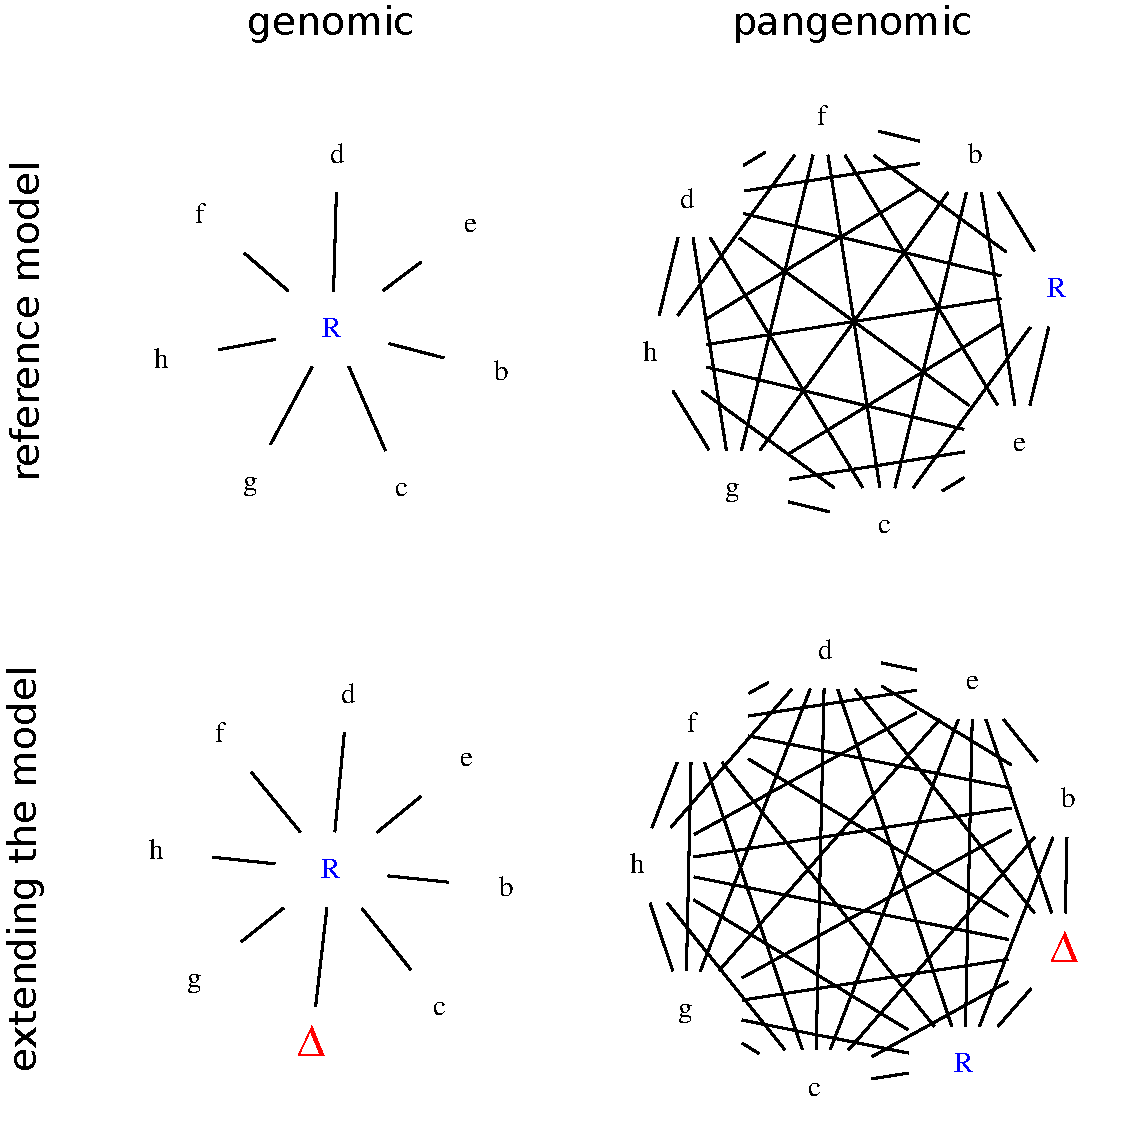
\includegraphics[width=0.9\textwidth]{figures/fig1.pdf}
    \caption{\label{fig:models} Genomic versus pangenomic sequence analysis}
%\textbf{A:} Bandage, adapted from \cite{Wick_2015} supplementary section~6.
%\textbf{B:} GfaViz, adapted from \cite{Gonnella_2018} supplementary figure~S4.
\end{figure}


%Each class of pangenomic model can be used as a basis to drive biological analyses.
%Implementations of particular analytical processes may produce or consume different types of pangenomic models.
%Methods to do so \todo{To do what?} are not fully equivalent.
%\todo[inline]{JME: I think this section should probably be expanded or cut}
%To provide perspective on the scope of these approaches, we consider their


%\subsection{Past reviews}

%\cite{computational2016computational}.
